\section{Swaptions as a missing link in asset allocation}
When constructing portfolio, there are many considerations and therefore many choice. 
Some of the thing we have to consider is the asset allocation, deriversification, rebalancing 
and risk management. This Section will be a motivation of why it is important to 
allocated to different asset class. The purpose it to see in which market situations
swaption perform better compared to other asset classes.
\\\\
But first a small introduction to portfolio construction. 
So a general  example is a 60/40 weight portfolio, where you allocated 60 percent to equities 
and 40 percent to fixed income. 
The investment belief in most portfolio is long beta, long duration, short volatility and short 
convexity. In other words the portfolio exception is to earn risk premium over the long term, 
where the asset have a long duration, to limited interest rate risk. And you want to be short in
volatility which means that you will sell option to gain risk premium. Secondly we note that we will expected 
a short convexity portfolio to under perform when interest rate are volatile. 
\begin{figure}[H]
    \centering
    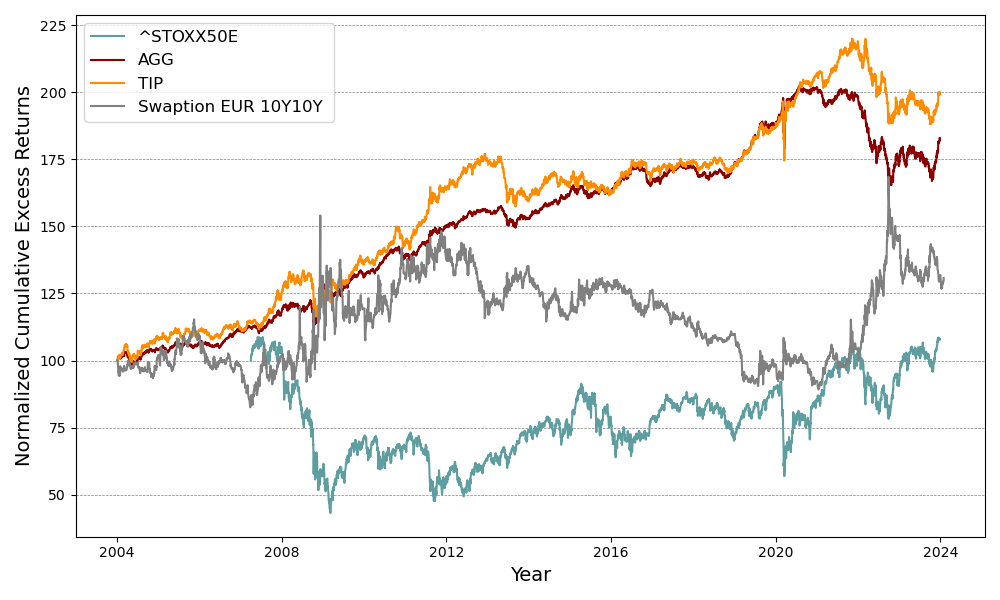
\includegraphics[width=0.9\textwidth]{/Users/nannaingemannohrt/Desktop/master_thesis/main/plots/2004_to_2024_plot.png}
    \caption{Comparison of Normalized Cululative Excess Return. Data source Citi Velocity 21.02.2024 
    and Yahoo Finance.}
    \label{fig:2004_2024}
\end{figure}
\noindent
Moving forward we will look a some market Data from Yahoo Finance and Citi Velocity. 
The purpose is two see how different asset class perform under some particular markets situations.
First we introduction to the different ticker, we will use to illustrated the different asset class. 
We will like to compare perform of the asset class equities, nominal bonds and inflation-linked bonds. 
The performs for the three asset class will be compared to swaption with ten years to expiry and a tenor
of ten years i euro, later in Section \ref{data_lab} the lingo of swaption will be covered. 
Below the chosen ticker are listed, with short explanation. Where the ticker STOXX50E represent equities, 
AGG represent nominal bond and TIP describe inflation-linked bonds.

\begin{itemize}
    \item \textbf{STOXX50E} \text{---}  index of 50 largest European equities.
    \item \textbf{AGG} \text{---}  index for US investment-grade bond. 
    \item \textbf{TIP} \text{---}  index for inflation-protected US-Treasury secitities.
    \end{itemize}
\noindent
Above in \autoref{fig:2004_2024} the three chosen ticker and the swaption development
is illustrated from 2004 to the start of 2024. 

\begin{figure}[H]
    \centering
    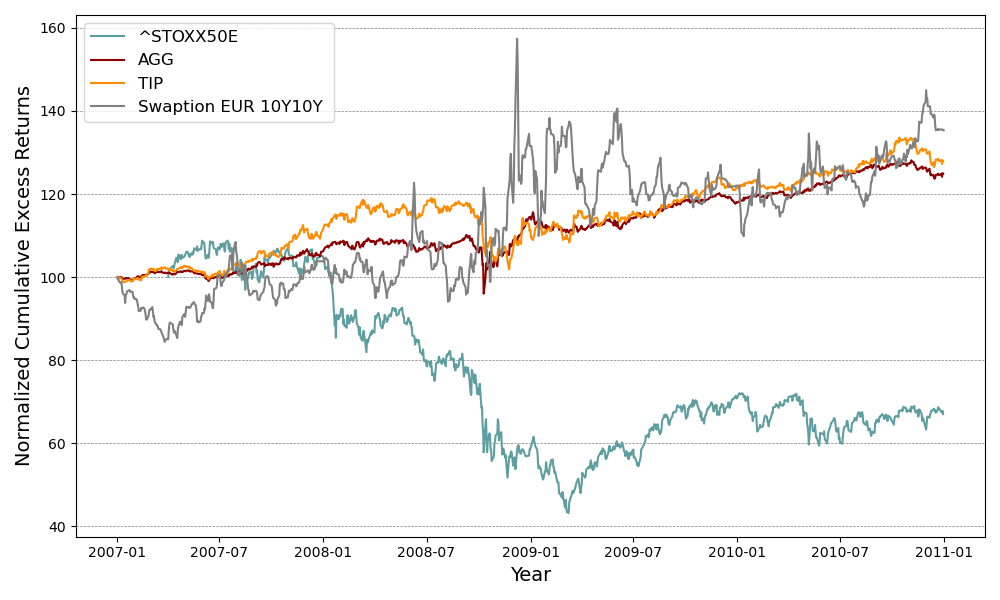
\includegraphics[width=0.9\textwidth]{/Users/nannaingemannohrt/Desktop/master_thesis/main/plots/2007_to_2011.png}
    \caption{}
    \label{fig:2007_2011}
\end{figure}
\noindent

\begin{figure}[H]
    \centering
    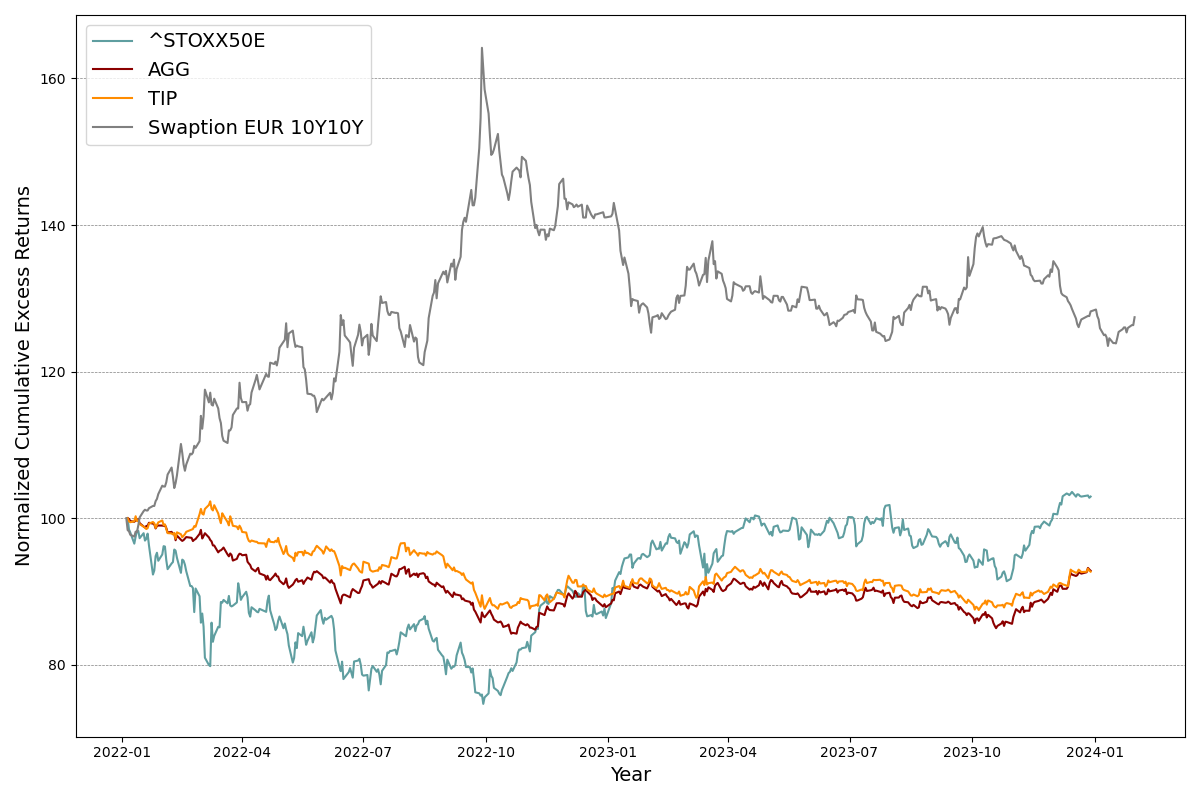
\includegraphics[width=0.9\textwidth]{/Users/nannaingemannohrt/Desktop/master_thesis/main/plots/2022_to_2024.png}
    \caption{}
    \label{fig:2007_2011}
\end{figure}
\noindent

